\documentclass{beamer}
%
\mode<presentation>
{
  \usetheme{fnbCD}
}

\usepackage[german]{babel}
\usepackage[latin1]{inputenc}
\usepackage{times}
\usepackage[T1]{fontenc}
\usepackage{multimedia}
\usepackage{hyperref}

\usepackage{mathdesign}
\usepackage[]{subfigure}
\usepackage{float}
\usepackage[]{graphicx}
%\usepackage[]{natbib}
\usepackage[]{amsmath}
\usepackage{dsfont}
\usepackage{color}
%Zur Darstellung von Code
%\usepackage[ruled,chapter]{algorithm}
\usepackage[]{algorithmic}
% Private Declarations
%\usepackage{psfrag}
\usepackage{multirow}
%\usepackage{latexsym}
%\usepackage{pstricks,pst-node}
%\usepackage{pst-blur}
%\usepackage{pstricks-add}
%Colors
%\definecolor{Pink}{rgb}{1.,0.75,0.8}
%\definecolor{fond}{RGB}{240,240,240}
%F�r Bibliography
\usepackage[fixlanguage]{babelbib}
\selectbiblanguage{german}
%\selectlanguage{english}
\usepackage{booktabs}
\usepackage{pgfplots}
\usepackage{rotating}
%\usepackage{longtable,tabu,booktabs}


%%%%%%%%%%%%%%%%%%%%%%%%%%%%%%%%%%%%%%%%%%%%%%%%%%%
%%%%%%%%%%%%%%%%%%%%%%%%%%%%%%%%%%%%%%%%%%%%%%%%%%%
%%                                               %%
%%  --- setup for the presentation ---           %%
%%                                               %%
%%%%%%%%%%%%%%%%%%%%%%%%%%%%%%%%%%%%%%%%%%%%%%%%%%%
%%%%%%%%%%%%%%%%%%%%%%%%%%%%%%%%%%%%%%%%%%%%%%%%%%%
%
%
%%%%%%%%%%%%%%%%%%%%%%%%%%%%%%%%%%%%%%%%%%%%%%%%%%
% Title and Subtitle
%%%%%%%%%%%%%%%%%%%%%%%%%%%%%%%%%%%%%%%%%%%%%%%%%%
%
% usage:   \title[short title]{title}
%
% short title necessary only for long titles, because optionally 
% goes to footer line


\title[Masterthesis ]{\small{Implementierung und Untersuchung \\einer hoch effizienten Methode \\zur Druck-Geschwindigkeits-Kopplung}}

\subtitle{\small{Masterthesis}}


%%%%%%%%%%%%%%%%%%%%%%%%%%%%%%%%%%%%%%%%%%%%%%%%%%
% Authors and Institute
%%%%%%%%%%%%%%%%%%%%%%%%%%%%%%%%%%%%%%%%%%%%%%%%%%
%
% usage: \author[short author]{author1\inst{1} \and \author2\inst{2}}
%
%        \institute[short institute]
%        {
%          \inst{1}
%             institute1
%          \and
%          \inst{2}
%             institute2
%        }
%
% short author/short institute necessary only for many authors,
% because optionally go to footer line
%
\author[Fabian Gabel ]
{{Fabian~Gabel }}

    %\institute[TU Darmstadt, FNB]
    %{
    %  \inst{1}%
    %  Fachgebiet Numerische Berechnungsverfahren\\
    %  im Maschinenbau, Raum 330
    %}


%%%%%%%%%%%%%%%%%%%%%%%%%%%%%%%%%%%%%%%%%%%%%%%%%%
% Date and conference name
%%%%%%%%%%%%%%%%%%%%%%%%%%%%%%%%%%%%%%%%%%%%%%%%%%
%
% usage:   \date[short date]{date}
%
% actually more useful for conference name
% short date necessary only if reused for footer line


\date[\today]
{Kolloquium, XX.XX.2015}

%%%%%%%%%%%%%%%%%%%%%%%%%%%%%%%%%%%%%%%%%%%%%%%%%%
% Subject
%%%%%%%%%%%%%%%%%%%%%%%%%%%%%%%%%%%%%%%%%%%%%%%%%%
%
% usage:   \subject{subject}
%
% this goes only into pdf-information catalogue so 
% rather optional


\subject{interne Bekanntmachung}

%%%%%%%%%%%%%%%%%%%%%%%%%%%%%%%%%%%%%%%%%%%%%%%%%%
% Misc
%%%%%%%%%%%%%%%%%%%%%%%%%%%%%%%%%%%%%%%%%%%%%%%%%%
%
% Uncomment the following if you would like to see 
% the Contents of your talk at the begin of every 
% section (appropriately highlighted)



% \AtBeginSubsection[]
% {
%   \begin{frame}<beamer>
%     \frametitle{Overview}
%     \tableofcontents[currentsection,currentsubsection]
%   \end{frame}
% }


% If itemize/enumerate environments are to be shown step by
% step generally, this command can be used

%\beamerdefaultoverlayspecification{<+->}

%\pgfdeclareimage[width=\paperwidth]{bg_alt_title}{fnbbeamer-bg-folie4x3-titel-foto-etch}
\pgfdeclareimage[width=\paperwidth]{bg_title}{fnbbeamer-bg-folie4x3-titel-etch}

\begin{document}
%%%%%%%%%%%%%%%%%%%%%%%%%%%%%%%%%%%%%%%%%%%%%%%%%%
% Title page
%%%%%%%%%%%%%%%%%%%%%%%%%%%%%%%%%%%%%%%%%%%%%%%%%%
% 
% usage: \fnbtitlepage{footerright}{alignment}{backgroundimage}

% standard title page is /fnbtitlepage which uses a different 
% backround image, puts the department url in left left bottom 
% corner and some other things.
%

%\fnbtitlepageintro{bg_alt_title}
\fnbtitlepage{\today}{bg_title}
%\fnbtitlepage{\today}{bg_alt_title}

% if you dont want the fnb-titlepage uncomment the following and
% comment out the \fnbtitlepage{}
%
%\begin{frame}
%   \titlepage
%\end{frame}

% choose navigation symbol appearance
% - [only frame symbol]
% - [vertical]
% - [horizontal]
% - {}    (empty hides nav symbols)

\setbeamertemplate{navigation symbols}[only frame symbol]

% placement redefinition because of FNB-Logo
\setbeamertemplate{sidebar right}[fnb theme]

% choose footer
 \setbeamertemplate{footline}[fnb theme]
% \setbeamertemplate{footline}[fnb theme noslidenumber]
% \setbeamertemplate{footline}[fnb theme simplefoot]
% \setbeamertemplate{footline}[fnb theme customfoot]{33}
% \setbeamertemplate{footline}[fnb theme customsimplefoot]{33}

 \begin{frame}
   \frametitle{Inhalt}

% % use
% % \tableofcontents[pausesections]
% % if you want to uncover the sections separately

   %\tableofcontents[pausesections]
   \tableofcontents
 \end{frame}


 \AtBeginSection[]
 {
 \begin{frame}<beamer>
   \frametitle{Inhalt}
     \tableofcontents[currentsection,currentsubsection]
     %\tableofcontents[pausesections]
   \end{frame}
 }

% %
% % Finally, observe to divide your talk in sections and subsections
% % on the one hand this ensures the correct entries in the table of
% % contents and on the other hand the presentation will be easier to 
% % transfer to other styles
% %
% %

% %%%%%%%%%%%%%%%%%%%%%%%%%%%%%%%%%%%%%%%%%%%%%%%%%%%
% %%%%%%%%%%%%%%%%%%%%%%%%%%%%%%%%%%%%%%%%%%%%%%%%%%%
% %%                                               %%
% %%  --- end of setup ---                         %%
% %%                                               %%
% %%%%%%%%%%%%%%%%%%%%%%%%%%%%%%%%%%%%%%%%%%%%%%%%%%%
% %%%%%%%%%%%%%%%%%%%%%%%%%%%%%%%%%%%%%%%%%%%%%%%%%%%

%%%%%%%%%%%%%%%%%%%%%%%%%%%%%%%%%%%%%%%%%%%%%%%%%%%%%%%%%%%%

\section{Motivation}
\begin{frame}

\frametitle{Motivation}
    \vspace{0.5cm}
    Challenges for CFD--applications:
    \begin{itemize}
    \item \small{Complex geometries and coupled multiphisics problems}
    \item \small{Short running time}
    \item \small{High accuracy}
    \end{itemize}

    \begin{columns}
        \begin{column}{6cm}
            \begin{figure}
            \centering
            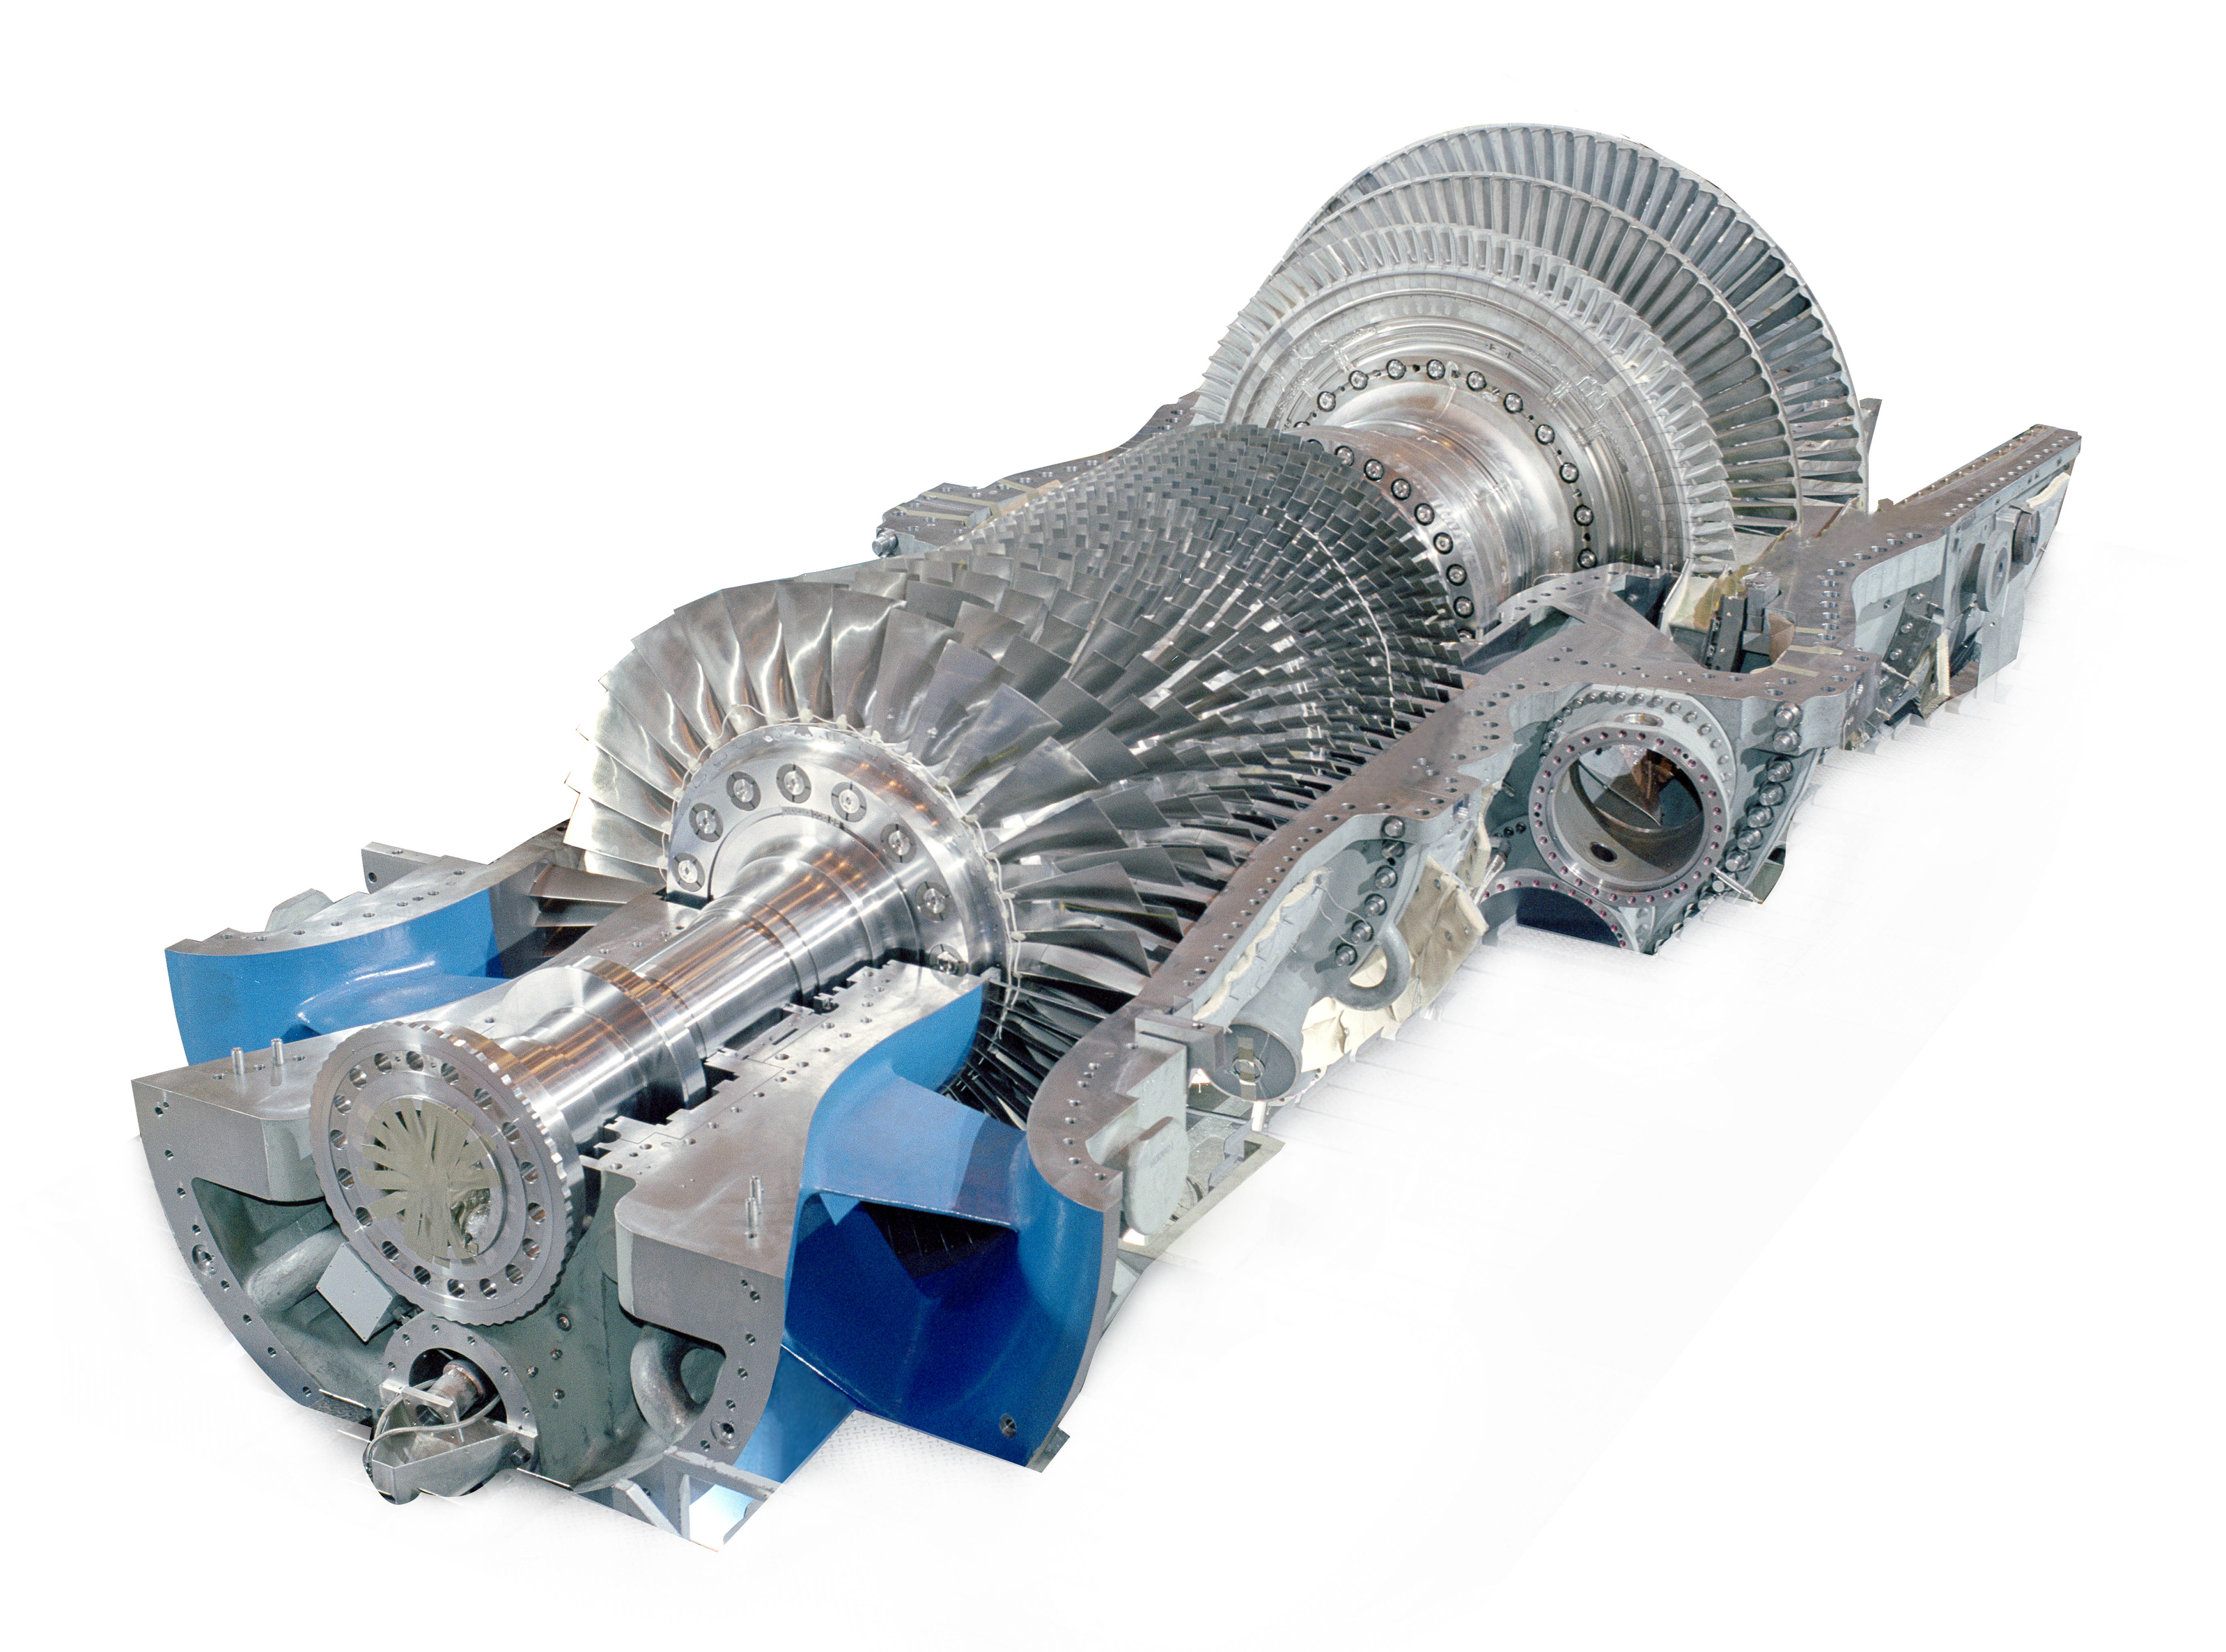
\includegraphics[width= 0.8\linewidth]{bilder/turbine.jpg}
            \caption{Gas turbine (VDI)}
            \end{figure}
        \end{column}
        \begin{column}{6cm}
            \begin{itemize}
                \item \small{Efficient, scalable algorithms}
                \item \small{Parallelisation}
                \item \small{Local block-refinement}
            \end{itemize}
        \end{column}
    \end{columns}

\end{frame}

%%%%%%%%%%%%%%%%%%%%%%%%%%%%%%%%%%%%%%%%%%%%%%%%%%%%%%%%%%%%

\begin{frame}

\frametitle{Motivation}
    Einfluss auf Laufzeit in wissenschaftlichen Codes:

    \begin{itemize}
    \item Flussberechnung
    \item L�sung linearer Gleichungssysteme
    \end{itemize}

    Effizienz des Gleichungsl�sers \(\rightarrow\) Effizienz des L�serprogramms

\end{frame}

%%%%%%%%%%%%%%%%%%%%%%%%%%%%%%%%%%%%%%%%%%%%%%%%%%%%%%%%%%%%

\begin{frame}

    \frametitle{PETSc}
    Portable, Extensible Toolkit for Scientific Computation
    \begin{itemize}
    \item R\&D Award (2009)
    \item Bibliothek f�r PDEs und Sparse--Matrix--Berechnungen
    \item Datenstrukturen f�r wissenschaftliche Codes (Vektoren, Matrizen, Index--Sets)
    \item Framework zur MPI--Parallelisierung
    \item hochskalierende Gleichungsl�ser und Pr�konditionierer
    \item weltweit am meisten eingesetzte numerische Softwarebibliothek
    \item CFD, Medizin, Wirtschaftsmodellierung, Strukturmechanik, Kernphysik, ...
    \end{itemize}

\end{frame}

%%%%%%%%%%%%%%%%%%%%%%%%%%%%%%%%%%%%%%%%%%%%%%%%%%%%%%%%%%%%

\begin{frame}

\frametitle{Aufgabenstellung}
    \begin{itemize}
    \item Sinnvoller Einsatz von PETSc zur Parallelisierung
    \item Anwendung auf einen L�ser f�r skalare Transportgleichungen
    \item h-refinement in Parallelisierung ber�cksichtigen
    \item Untersuchung der parallelen Effizienz der Applikation
    \end{itemize}
\end{frame}

%%%%%%%%%%%%%%%%%%%%%%%%%%%%%%%%%%%%%%%%%%%%%%%%%%%%%%%%%%%%

\section{Implementierung}

\begin{frame}
\frametitle{Gittergenerierung}
%\vspace{0.2cm}
\begin{columns}
\begin{column}{6cm}
\begin{itemize}
    \item Enwicklung Gittergenerator
    \begin{itemize}
        \item Gittergeometrie
        \item kartesische Gitterbl�cke
        \item Randbedingungen
    \end{itemize}
\end{itemize}
\end{column}
\begin{column}{6cm}
\begin{figure}
\centering
%\includegraphics[trim=3cm 24cm 0cm 2cm,width=1.2\linewidth]{bilder/grid}
\end{figure}
\end{column}
\end{columns}

\end{frame}

%%%%%%%%%%%%%%%%%%%%%%%%%%%%%%%%%%%%%%%%%%%%%%%%%%%%%%%%%%%%

\begin{frame}

\frametitle{Behandlung von Blockr�ndern}
\vspace{0.2cm}

\begin{figure}
\centering
%\includegraphics[width=0.4\textwidth]{bilder/ghostcells}
\end{figure}

    \begin{columns}
        \begin{column}{1cm}
        \end{column}
        \begin{column}{5cm}
        \tiny{Ansatz nach Lange et al.}
            \begin{figure}
                %\centering
                %\includegraphics[width=1.0\textwidth]{bilder/multigrid}
            \end{figure}
        \end{column}

        \begin{column}{5cm}
        \tiny{Ansatz nach Lilek et al.}
            \begin{figure}
                %\centering
              %\includegraphics[width=0.7\textwidth]{bilder/peric}
            \end{figure}
        \end{column}
    \end{columns}

\end{frame}

%%%%%%%%%%%%%%%%%%%%%%%%%%%%%%%%%%%%%%%%%%%%%%%%%%%%%%%%%%%%

\begin{frame}
\frametitle{Preprocessing}
%\begin{columns}

%    \begin{column}{6cm}
    \begin{itemize}
        \item Preprocessing zur Ermittlung der Nachbarschaftsbeziehungen
        \begin{itemize}
            \item Globale Indexierung
            \item Teilgrenzfl�chen
        \end{itemize}
    \end{itemize}
%    \end{column}

    %\begin{column}{6cm}
    \begin{figure}
        \centering
        %\includegraphics[width=0.5\textwidth]{bilder/peric}
    \end{figure}
    %\end{column}

%\end{columns}

\end{frame}

%%%%%%%%%%%%%%%%%%%%%%%%%%%%%%%%%%%%%%%%%%%%%%%%%%%%%%%%%%%%

\begin{frame}

\frametitle{L�serprogramm}
\begin{itemize}

    \item Parallele L�sung der skalaren Transportgleichung
    \item Ortsdiskretisierung mittels Finite--Volumen--Ansatz
    \begin{itemize}
        \item UDS (implizit,explizit) + CDS (explizit) -- Konvektiv
        \item Zentraldifferenzen -- Diffusiv
        \item Verz�gerte Korrektur
    \end{itemize}

    \item Finite--Differenzen Zeitdiskretisierung
    \begin{itemize}
        \item Implizites Einschrittverfahren
    \end{itemize}

\end{itemize}

\end{frame}

%%%%%%%%%%%%%%%%%%%%%%%%%%%%%%%%%%%%%%%%%%%%%%%%%%%%%%%%%%%%

\begin{frame}
\frametitle{Einbindung von PETSc}
\vspace{0.2cm}
\small{Austausch von Variablenwerten benachbarter Bl�cke (Scatter--Routinen)}

\begin{figure}
\centering
%\includegraphics[width=0.8\textwidth]{bilder/vectoarr}
\end{figure}

\end{frame}

%%%%%%%%%%%%%%%%%%%%%%%%%%%%%%%%%%%%%%%%%%%%%%%%%%%%%%%%%%%%

\begin{frame}

\frametitle{Einbindung von PETSc}
\vspace{0.2cm}
\small{Parallele Matrixassemblierung (globale Systemmatrix)}

\begin{figure}
\centering
%\includegraphics[width=0.6\textwidth]{bilder/matrix}
\end{figure}

\end{frame}

%%%%%%%%%%%%%%%%%%%%%%%%%%%%%%%%%%%%%%%%%%%%%%%%%%%%%%%%%%%%

\section{Verifikation}
\begin{frame}

\frametitle{Verifikation}
\vspace{0.2cm}
\begin{itemize}
    \item \small{Konsistenzordnung 2 -- �rtlich, 1 -- zeitlich}
    \item \small{Methode der Manufactured Solutions}
    \item \small{\( \phi^m (t,x,y,z )=( 2\sin (x^2\pi)+3\cos (y^2\pi)+5\sin (z^2\pi ) )\exp (-t ) \)}
\end{itemize}
\vspace{0.2cm}

\pgfplotsset{
    tick label style={font=\tiny}
    }
\begin{figure}
\centering
\begin{tikzpicture}
\begin{loglogaxis}[
    %small,
    width=7cm,
    ylabel=Fehler,
    xtick={1,2,4,8},
    xticklabels={${1h_x\text{, }1h_t}$,$2h_x\text{, }4h_t$,$4h_x\text{, }16h_t$,$8h_x\text{, }64h_t$},
    grid=major,
    legend style={ cells={anchor=east}, legend pos=outer north east, },
    ]
    \addplot coordinates {
        (1, 2.70705849688271719E-004) 
        (2, 1.11517924567996834E-003) 
        (4, 4.41834118871322311E-003)
        (8, 1.67582264349951486E-002) };
    \addlegendentry{beob. Fehler};
    \addplot[red] coordinates {
        (1, 0.0002618472880467992) 
        (2, 0.0010473891521871968) 
        (4, 0.0041895566087487872)
        (8, 1.67582264349951486E-002) };
    \addlegendentry{id. Fehler};

\end{loglogaxis}
\end{tikzpicture}
\end{figure}

\end{frame}

%%%%%%%%%%%%%%%%%%%%%%%%%%%%%%%%%%%%%%%%%%%%%%%%%%%%%%%%%%%%

\section{Untersuchung der Effizienz}
\begin{frame}

\frametitle{Benchmark als Voruntersuchung}
\vspace{0.2cm}
\small{STREAM-Benchmark (Triad) zur Voruntersuchung auf Multiprozessorsystem \textit{texas}}

\begin{figure}
\centering
%\includegraphics[width=0.8\textwidth]{bilder/konfig}
\end{figure}

\end{frame}

%%%%%%%%%%%%%%%%%%%%%%%%%%%%%%%%%%%%%%%%%%%%%%%%%%%%%%%%%%%%
\begin{frame}

\frametitle{Benchmark als Voruntersuchung}
\vspace{0.2cm}

\small{Einflussfaktoren: Bandbreite \(\leftrightarrow\) Latenzzeit}

%   \begin{columns}
%   \begin{column}{8cm}
%       \begin{figure}
%       \centering
%       \begin{tikzpicture}
%       \begin{axis}[
%           ylabel=Bandbreite MB/s,
%           xtick={1,2,3,4},
%           xticklabels={$a$,$b$,$c$,$d$},
%           xlabel=Verwendete Konfiguration,
%           grid=major,
%           width=6cm,
%           legend style={ cells={anchor=east}, legend pos=outer north east, }
%           ]
%           \addplot file {inputfiles/benchmark/bench.1};
%               \addlegendentry {1 P};
%           \addplot file {inputfiles/benchmark/bench.2};
%               \addlegendentry {2 P};
%           \addplot file {inputfiles/benchmark/bench.4};
%               \addlegendentry {4 P};
%           \addplot file {inputfiles/benchmark/bench.8};
%               \addlegendentry {8 P};
%           \addplot file {inputfiles/benchmark/bench.16};
%               \addlegendentry {16 P};
%           \addplot file {inputfiles/benchmark/bench.32};
%               \addlegendentry {32 P};
%           \addplot file {inputfiles/benchmark/bench.64};
%               \addlegendentry {64 P};
%       \end{axis}
%       \end{tikzpicture}
%       \label{fig:bench}
%       \end{figure}
%   \end{column}
%   \begin{column}{4cm}
%   %\includegraphics[width=0.8\linewidth]{bilder/16Konfig}
%   \end{column}
%   \end{columns}

\end{frame}

%%%%%%%%%%%%%%%%%%%%%%%%%%%%%%%%%%%%%%%%%%%%%%%%%%%%%%%%%%%%

\begin{frame}
\frametitle{Numerische Effizienz}
\vspace{0.2cm}
    \begin{itemize}
        \item \small{station�res Problem mit \(2e6\) Unbekannten}
        \item \small{Effizienz der L�sung eines Gleichungssystems}
    \end{itemize}
%       \begin{figure}
%       \centering
%       \begin{tikzpicture}
%       \begin{semilogxaxis}
%           [
%           width=7cm,
%           ylabel=numerische Effizienz,
%           ymin=0.5,
%           ymax=1.4,
%           xlabel=Anzahl Prozessoren,
%           xtick={1,2,4,8,16,32,64},
%           xticklabels={1,2,4,8,16,32,64},
%           grid=major,
%           legend style={ cells={anchor=east}, legend pos=outer north east, }
%           ]
%           \addplot file {inputfiles/numericalEfficiency/numericalEfficiency_bjacobi.128.out};
%               \addlegendentry {Block--Jakobi};
%           \addplot file {inputfiles/numericalEfficiency/numericalEfficiency_ml.128.out};
%               \addlegendentry {AMG};
%       \end{semilogxaxis}
%       \end{tikzpicture}
%       \end{figure}

\end{frame}

%%%%%%%%%%%%%%%%%%%%%%%%%%%%%%%%%%%%%%%%%%%%%%%%%%%%%%%%%%%%

\begin{frame}
\frametitle{Parallele Effizienz}
\vspace{0.2cm}
\small{Anzahl Bl�cke bzw. innerer Iterationen konstant gehalten}
\vspace{0.5cm}

%\begin{columns}
%\pgfplotsset{
%    tick label style={font=\small}
%    }
%    \begin{column}{5cm}
%    \centering
%    \begin{tikzpicture}
%    \begin{axis}[
%        title=Block--Jakobi,
%        ymin=0,
%        ymax=1.1,
%        grid=major,
%        width=5cm,
%        ylabel=parallele Effizienz,
%        xtick={1,2,3,4},
%        xticklabels={$a$,$b$,$c$,$d$},
%        ytick={0,0.2,0.4,0.6,0.8,1},
%        xlabel=Konfiguration
%        %legend style={ cells={anchor=east}, legend pos=outer north east, }
%        ]
%        \addplot file {inputfiles/parallelEfficiency_new/parallelEfficiency_bjacobi_new.128.1.out};
%            %\addlegendentry {1 Prozessor};
%        \addplot file {inputfiles/parallelEfficiency_new/parallelEfficiency_bjacobi_new.128.2.out};
%            %\addlegendentry {2 Prozessoren};
%        \addplot file {inputfiles/parallelEfficiency_new/parallelEfficiency_bjacobi_new.128.4.out};
%            %\addlegendentry {4 Prozessoren};
%        \addplot file {inputfiles/parallelEfficiency_new/parallelEfficiency_bjacobi_new.128.8.out};
%            %\addlegendentry {8 Prozessoren};
%        \addplot file {inputfiles/parallelEfficiency_new/parallelEfficiency_bjacobi_new.128.16.out};
%            %\addlegendentry {16 Prozessoren};
%        \addplot file {inputfiles/parallelEfficiency_new/parallelEfficiency_bjacobi_new.128.32.out};
%            %\addlegendentry {32 Prozessoren};
%        \addplot file {inputfiles/parallelEfficiency_new/parallelEfficiency_bjacobi_new.128.64.out};
%            %\addlegendentry {64 Prozessoren};
%    \end{axis}
%    \end{tikzpicture}
%%    \caption{\(2e6\) KVs}
%    \end{column}
%    \begin{column}{6cm}
%    \centering
%    \begin{tikzpicture}
%    \begin{axis}[
%        title=AMG,
%        ymin=0,
%        ymax=1.1,
%        grid=major,
%        width=5cm,
%        %ylabel=parallele Effizienz,
%        xtick={1,2,3,4},
%        xticklabels={$a$,$b$,$c$,$d$},
%        ytick={0,0.2,0.4,0.6,0.8,1},
%        xlabel=Konfiguration,
%        legend style={ cells={anchor=east}, legend pos=outer north east, }
%        ]
%        \addplot file {inputfiles/parallelEfficiency/parallelEfficiency_ml.128.1.out};
%            \addlegendentry {1 P};
%        \addplot file {inputfiles/parallelEfficiency/parallelEfficiency_ml.128.2.out};
%            \addlegendentry {2 P};
%        \addplot file {inputfiles/parallelEfficiency/parallelEfficiency_ml.128.4.out};
%            \addlegendentry {4 P};
%        \addplot file {inputfiles/parallelEfficiency/parallelEfficiency_ml.128.8.out};
%            \addlegendentry {8 P};
%        \addplot file {inputfiles/parallelEfficiency/parallelEfficiency_ml.128.16.out};
%            \addlegendentry {16 P};
%        \addplot file {inputfiles/parallelEfficiency/parallelEfficiency_ml.128.32.out};
%            \addlegendentry {32 P};
%        \addplot file {inputfiles/parallelEfficiency/parallelEfficiency_ml.128.64.out};
%            \addlegendentry {64 P};
%    \end{axis}
%    \end{tikzpicture}
%    \end{column}
%\end{columns}
%%\vspace{0.5cm}

\end{frame}

%%%%%%%%%%%%%%%%%%%%%%%%%%%%%%%%%%%%%%%%%%%%%%%%%%%%%%%%%%%%

\begin{frame}
\frametitle{Strong Scaling}
\vspace{0.2cm}
\small{Testfall mit insgesamt \(2e6\) Unbekannten; 8 gerechntete Zeitschritte}

\begin{figure}[h!]
\centering
\begin{tikzpicture}
\begin{loglogaxis}
    [
    width=7cm,
    ylabel=SpeedUp,
    xlabel=Anzahl Prozessoren,
    xtick={1,2,4,8,16,32,64},
    ytick={1,2,4,8,16,32,64}, xticklabels={1,2,4,8,16,32,64},
    yticklabels={1,2,4,8,16,32,64},
    grid=major,
    legend style={ cells={anchor=east}, legend pos=outer north east, }
    ]
    \addplot file {inputfiles/speedup/speedup_bjacobi.128};
        \addlegendentry {Block--Jakobi};
    \addplot file {inputfiles/speedup/speedup_ml.128};
        \addlegendentry {AMG};
\end{loglogaxis}
\end{tikzpicture}
%\caption{SpeedUp des Programms f"ur einen vorgegebenen Testfall}
%\label{fig:speedup}
\end{figure}

\end{frame}

%%%%%%%%%%%%%%%%%%%%%%%%%%%%%%%%%%%%%%%%%%%%%%%%%%%%%%%%%%%%

\begin{frame}

\frametitle{Weak Scaling}
\vspace{0.2cm}
\small{Testfall mit \(2e6\) Unbekannten pro Prozessor, 8 gerechnete Zeitschritte}

\begin{figure}[h!]
\centering
\begin{tikzpicture}
\begin{semilogxaxis}
    [
    width=7cm,
    ylabel=Laufzeit in s,
    xlabel=Anzahl Prozessoren,
    %ytick={100,300,500,1000},
    %yticklabels={100,300,500,1000},
    xtick={1,2,4,8,16,32,64},
    grid=major,
    xticklabels={1,2,4,8,16,32,64},
    grid=major,
    legend style={ cells={anchor=east}, legend pos=outer north east, }
    ]
    \addplot file {inputfiles/weakscaling/weakscaling_bjacobi.128};
        \addlegendentry {Block--Jakobi};
    \addplot file {inputfiles/weakscaling/weakscaling_ml.128};
        \addlegendentry {AMG};
\end{semilogxaxis}
\end{tikzpicture}
%\caption{Laufzeitentwicklung der Programmausf"uhrung in der Untersuchung des \textit{weak scaling}}
%\label{fig:weak}
\end{figure}

\end{frame}

%%%%%%%%%%%%%%%%%%%%%%%%%%%%%%%%%%%%%%%%%%%%%%%%%%%%%%%%%%%%

\section{Fazit und Ausblick}

\begin{frame}
\frametitle{Fazit und Ausblick}
\vspace{0.2cm}
\begin{itemize}
    \item paralleler L�ser f�r skalare Transportgleichung
    \item station�re/instation�re Probleme
    \item 3d blockstrukturierte Gitter (M�glichkeit zu h-refinement)
    \item Kopplung der Bl�cke nach Ansatz von Lilek et al.
    \item Benchmark Untersuchungen
    \item Skalierbarkeit der Applikation
\end{itemize}
Weiterf�hrung:
\begin{itemize}
    \item Str�mungsl�ser
    \item Potential hybrider Parallelisierung
    \item Field--Interlacing 
\end{itemize}

\end{frame}
%%%%%%%%%%%%%%%%%%%%%%%%%%%%%%%%%%%%%%%%%%%%%%%%%%%%%%%%%%%%
%%%%%%%%%%%%%%%%%%%%%%%%%%%%%%%%%%%%%%%%%%%%%%%%%%%%%%%%%%%%


 
\end{document}




